\section{Image Collection And Annotation}

\label{sec:image}

% ===================First Paragraph===============================
% how many query image; how many aerial images; where is the photo taken

% ===================Second Paragraph===============================
% the annotation: the scale and location of query image on the aerial map.  The point correspondence between two images

\begin{figure}[ht] 
\centering
\subfigure[{}]{ 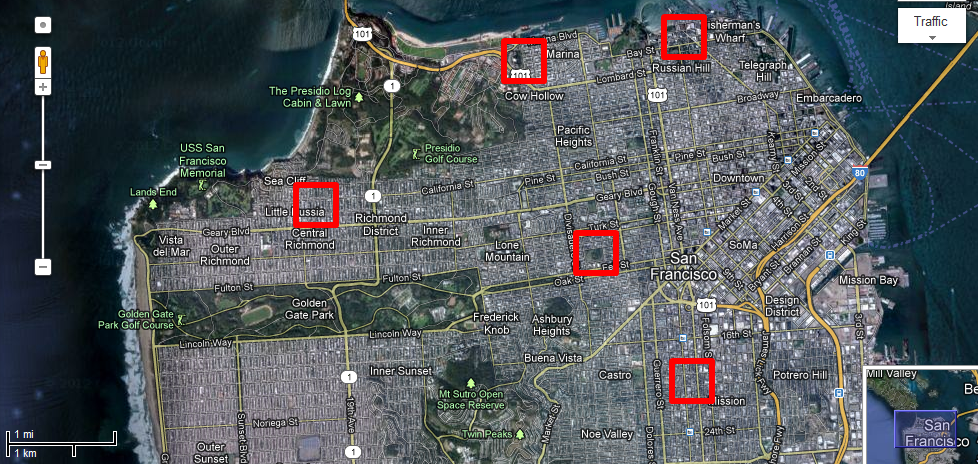
\includegraphics[width=0.4\textwidth]{pictures/collection-a} \label{collection-a} }
\subfigure[{}]{ 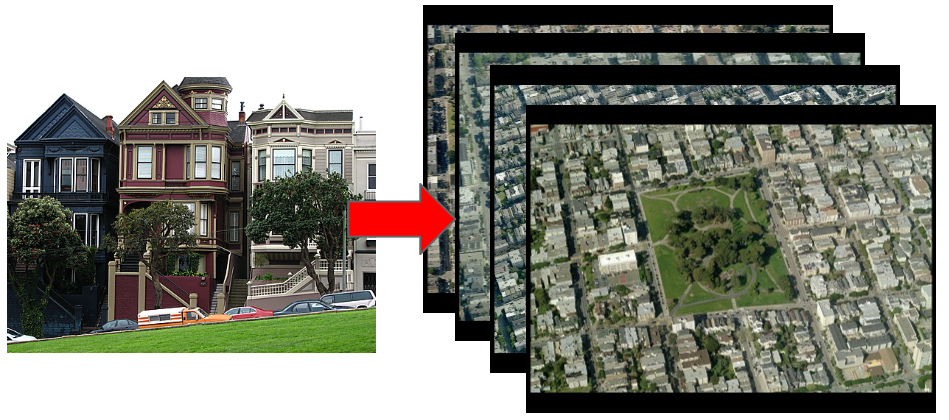
\includegraphics[width=0.4\textwidth]{pictures/collection-b} \label{collection-b} }
\caption[]{\subref{collection-a} We evaluate matching on the 5 areas bounded by red boxes. \subref{collection-b} Each query image matches to 4 aerial images in one area.}
\label{dataset}
\end{figure}
